\sect{Experiment}

FPGA data was collected on a system with a Xilinx Alveo U280 PCIe card,
containing a XCU280 FPGA and $\SI{8}{\giga\byte}$ of on-chip high-bandwidth
memory (HBM) \autocite{u280}. The CPU baseline was collected on a system with an
Intel Core i9-9900 CPU and $\SI{32}{\giga\byte}$ of installed RAM running Ubuntu
20.04 LTS.


\subsect{Tree Fanout}

\begin{figure}[H]
	\centering
	\begin{subfigure}{7.5cm}
		\centering
		\input{pgfplots/cpu-sequential-insertion}
		\caption{Sequential Insertion}
		\label{fig:cpu-sequential-insertion}
	\end{subfigure}
	\begin{subfigure}{7.5cm}
		\centering
		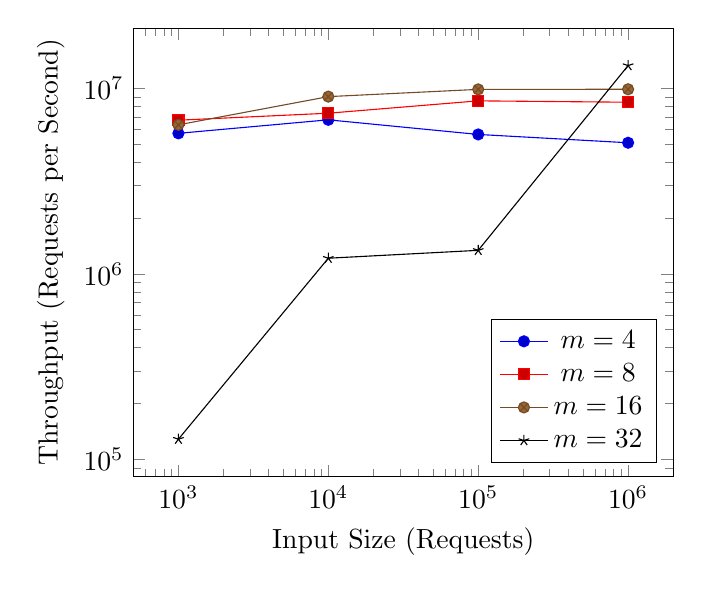
\begin{tikzpicture}
	\begin{axis}
		[
			xlabel={Input Size (Requests)},
			ylabel={Throughput (Requests per Second)},
			legend pos=south east,
			domain=1:1000000,
			xmode=log,
			ymode=log,
		]
		\addplot+[cycle list name=color list]
			coordinates {
				(1000, 5730659.02578797)
				(10000, 6777363.60555744)
				(100000, 5652112.47703829)
				(1000000, 5097827.30600218)
			};
		\addlegendentry{$m=4$}
		\addplot+[cycle list name=color list]
			coordinates {
				(1000, 6745362.56323777)
				(10000, 7358351.72921266)
				(100000, 8577616.70919735)
				(1000000, 8432751.96535826)
			};
		\addlegendentry{$m=8$}
		\addplot+[cycle list name=color list]
			coordinates {
				(1000, 6369426.75159236)
				(10000, 9039548.02259887)
				(100000, 9890463.12093564)
				(1000000, 9903416.92642504)
			};
		\addlegendentry{$m=16$}
		\addplot+[cycle list name=color list]
			coordinates {
				(1000, 128530.57421034)
				(10000, 1215583.78411232)
				(100000, 1340572.42442523)
				(1000000, 13292569.4536754)
			};
		\addlegendentry{$m=32$}
	\end{axis}
\end{tikzpicture}

		\caption{Random Insertion}
		\label{fig:cpu-random-insertion}
	\end{subfigure}
	\caption{CPU Insertion}
	\label{fig:cpu-insertion}
\end{figure}

\begin{figure}[H]
	\centering
	\begin{subfigure}{7.5cm}
		\centering
		\begin{tikzpicture}[scale=0.8]
	\begin{axis}
		[
			xlabel={Input Size (Requests)},
			ylabel={Throughput (Requests per Second)},
			legend pos=north west,
			domain=1:1000000,
			xmode=log,
			ymode=log,
			cycle list name=rainbow,
		]
		\addplot coordinates {
			(1000, 2633311.38907176)
			(10000, 22321428.5714286)
			(100000, 217273221.075503)
			(1000000, 1724137931.03448)
		};
		\addlegendentry{$m=4$}
		\addplot coordinates {
			(1000, 2857142.85714286)
			(10000, 26195153.8965291)
			(100000, 216684723.726977)
			(1000000, 1746724890.82969)
		};
		\addlegendentry{$m=8$}
		\addplot coordinates {
			(1000, 2756719.50379049)
			(10000, 22209883.3981122)
			(100000, 213789417.423837)
			(1000000, 1839080459.77011)
		};
		\addlegendentry{$m=16$}
		\addplot coordinates {
			(1000, 2818886.53981677)
			(10000, 26809651.4745308)
			(100000, 237107291.0492)
			(1000000, 2285714285.71429)
		};
		\addlegendentry{$m=32$}
	\end{axis}
\end{tikzpicture}

		\caption{Sequential Insertion}
		\label{fig:fpga-sequential-insertion}
	\end{subfigure}
	\begin{subfigure}{7.5cm}
		\centering
		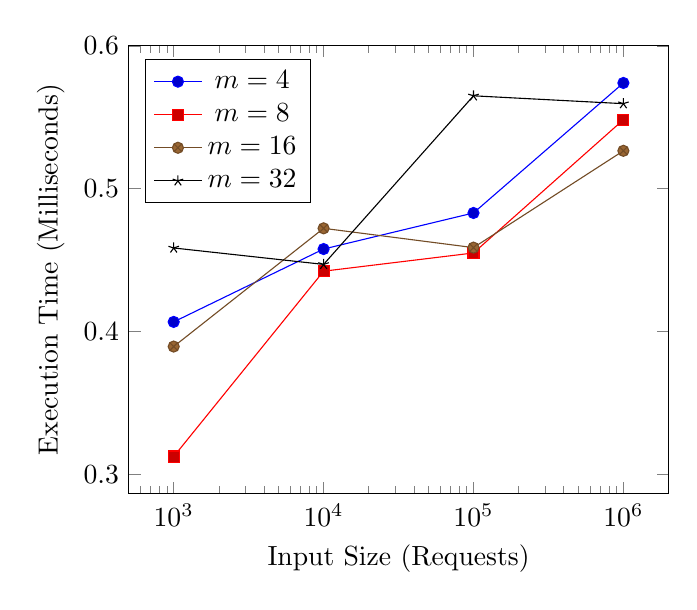
\begin{tikzpicture}
	\begin{axis}
		[
			xlabel={Input Size (Requests)},
			ylabel={Execution Time (Milliseconds)},
			legend pos=north west,
			domain=1:1000000,
			xmode=log,
		]
		\addplot+[cycle list name=color list]
			coordinates {
				(1000, 0.40675)
				(10000, 0.45775)
				(100000, 0.483)
				(1000000, 0.574)
			};
		\addlegendentry{$m=4$}
		\addplot+[cycle list name=color list]
			coordinates {
				(1000, 0.3125)
				(10000, 0.44225)
				(100000, 0.455)
				(1000000, 0.54825)
			};
		\addlegendentry{$m=8$}
		\addplot+[cycle list name=color list]
			coordinates {
				(1000, 0.3895)
				(10000, 0.47225)
				(100000, 0.45875)
				(1000000, 0.5265)
			};
		\addlegendentry{$m=16$}
		\addplot+[cycle list name=color list]
			coordinates {
				(1000, 0.4585)
				(10000, 0.447)
				(100000, 0.565)
				(1000000, 0.5595)
			};
		\addlegendentry{$m=32$}
	\end{axis}
\end{tikzpicture}

		\caption{Random Insertion}
		\label{fig:fpga-random-insertion}
	\end{subfigure}
	\caption{FPGA Insertion}
	\label{fig:fpga-insertion}
\end{figure}

\begin{figure}[H]
	\centering
	\begin{subfigure}{7.5cm}
		\centering
		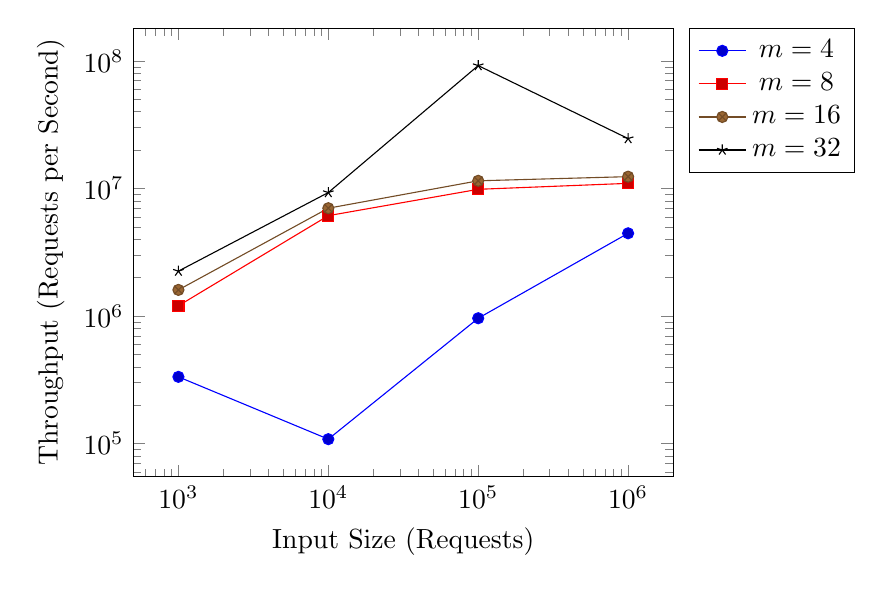
\begin{tikzpicture}
	\begin{axis}
		[
			xlabel={Input Size (Requests)},
			ylabel={Throughput (Requests per Second)},
			legend pos=outer north east,
			domain=1:1000000,
			xmode=log,
			ymode=log,
		]
		\addplot+[cycle list name=color list]
			coordinates {
				(1000, 333527.891269908)
				(10000, 108242.680088759)
				(100000, 960861.700773254)
				(1000000, 4455613.18148604)
			};
		\addlegendentry{$m=4$}
		\addplot+[cycle list name=color list]
			coordinates {
				(1000, 1203731.56786037)
				(10000, 6125574.27258806)
				(100000, 9856829.55077499)
				(1000000, 10976496.5767051)
			};
		\addlegendentry{$m=8$}
		\addplot+[cycle list name=color list]
			coordinates {
				(1000, 1603206.41282565)
				(10000, 7008936.39390223)
				(100000, 11494252.8735632)
				(1000000, 12389501.1367367)
			};
		\addlegendentry{$m=16$}
		\addplot+[cycle list name=color list]
			coordinates {
				(1000, 2249718.78515186)
				(10000, 9300162.75284818)
				(100000, 92059838.8952819)
				(1000000, 24630086.8826315)
			};
		\addlegendentry{$m=32$}
	\end{axis}
\end{tikzpicture}

		\caption{Sequential Search}
		\label{fig:cpu-sequential-search}
	\end{subfigure}
	\begin{subfigure}{7.5cm}
		\centering
		\input{pgfplots/cpu-random-search}
		\caption{Random Search}
		\label{fig:cpu-random-search}
	\end{subfigure}
	\caption{CPU Search}
	\label{fig:cpu-search}
\end{figure}

\begin{figure}[H]
	\centering
	\begin{subfigure}{7.5cm}
		\centering
		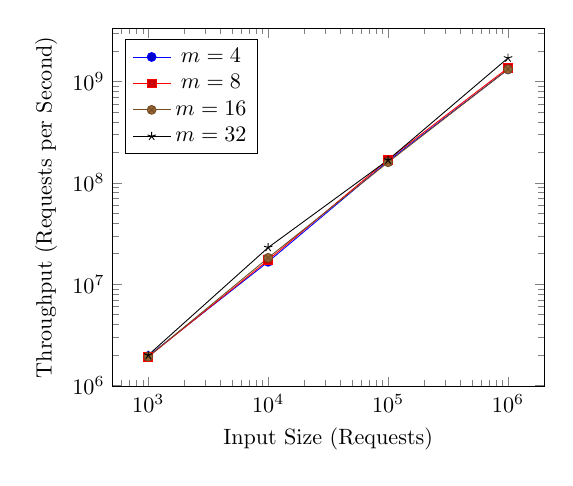
\begin{tikzpicture}[scale=0.8]
	\begin{axis}
		[
			xlabel={Input Size (Requests)},
			ylabel={Throughput (Requests per Second)},
			legend pos=north west,
			domain=1:1000000,
			xmode=log,
			ymode=log,
		]
		\addplot+[cycle list name=color list]
			coordinates {
				(1000, 1954079.14020518)
				(10000, 16638935.1081531)
				(100000, 164203612.479475)
				(1000000, 1321440370.0033)
			};
		\addlegendentry{$m=4$}
		\addplot+[cycle list name=color list]
			coordinates {
				(1000, 1914791.7663954)
				(10000, 17301038.0622837)
				(100000, 169923534.409516)
				(1000000, 1367053998.63295)
			};
		\addlegendentry{$m=8$}
		\addplot+[cycle list name=color list]
			coordinates {
				(1000, 1920307.24915987)
				(10000, 18223234.6241458)
				(100000, 159808230.123851)
				(1000000, 1322314049.58678)
			};
		\addlegendentry{$m=16$}
		\addplot+[cycle list name=color list]
			coordinates {
				(1000, 1997004.49326011)
				(10000, 23014959.7238205)
				(100000, 168491996.63016)
				(1000000, 1710863986.31309)
			};
		\addlegendentry{$m=32$}
	\end{axis}
\end{tikzpicture}

		\caption{Sequential Search}
		\label{fig:fpga-sequential-search}
	\end{subfigure}
	\begin{subfigure}{7.5cm}
		\centering
		\begin{tikzpicture}[scale=0.8]
	\begin{axis}
		[
			xlabel={Input Size (Requests)},
			ylabel={Throughput (Requests per Second)},
			legend pos=north west,
			domain=1:1000000,
			xmode=log,
			ymode=log,
			cycle list name=rainbow6,
		]
		\addplot coordinates {
			(1000, 1974333.66238894)
			(10000, 16380016.3800164)
			(100000, 160000000)
			(1000000, 1328903654.48505)
		};
		\addlegendentry{$m=4$}
		\addplot coordinates {
			(1000, 2208724.46162341)
			(10000, 16743407.2833822)
			(100000, 164001640.0164)
			(1000000, 1391788448.15588)
		};
		\addlegendentry{$m=8$}
		\addplot coordinates {
			(1000, 2022244.69160768)
			(10000, 16488046.1665293)
			(100000, 164744645.799012)
			(1000000, 1342732460.55723)
		};
		\addlegendentry{$m=16$}
		\addplot coordinates {
			(1000, 1619433.19838057)
			(10000, 16090104.5856798)
			(100000, 130975769.482646)
			(1000000, 1377410468.31956)
		};
		\addlegendentry{$m=32$}
	\end{axis}
\end{tikzpicture}

		\caption{Random Search}
		\label{fig:fpga-random-search}
	\end{subfigure}
	\caption{FPGA Search}
	\label{fig:fpga-search}
\end{figure}


\subsect{Workload Balance}

\begin{figure}[H]
	\centering
	\begin{tikzpicture}
	\begin{axis}
		[
			xlabel={Request Count},
			ylabel={Execution Time ($\unit{\milli\second}$)},
			legend pos=south east,
			domain=1:1000000,
			xmode=log,
			ymode=log,
		]
		\addplot+[cycle list name=color list]
			coordinates {
				(1000, 2.626)
				(10000, 206.79625)
				(100000, 11410.7)
				(1000000, 117235.5)
			};
		\addlegendentry{$\SI{20}{\percent}$ Read, $\SI{80}{\percent}$ Write}
		\addplot+[cycle list name=color list]
			coordinates {
				(1000, 1.731)
				(10000, 140.31525)
				(100000, 8097.0275)
				(1000000, 91322.3)
			};
		\addlegendentry{$\SI{40}{\percent}$ Read, $\SI{60}{\percent}$ Write}
		\addplot+[cycle list name=color list]
			coordinates {
				(1000, 1.20775)
				(10000, 89.748)
				(100000, 4969.515)
				(1000000, 52228.5)
			};
		\addlegendentry{$\SI{60}{\percent}$ Read, $\SI{40}{\percent}$ Write}
		\addplot+[cycle list name=color list]
			coordinates {
				(1000, 0.76375)
				(10000, 44.85)
				(100000, 2507.505)
				(1000000, 28785.65)
			};
		\addlegendentry{$\SI{80}{\percent}$ Read, $\SI{20}{\percent}$ Write}
	\end{axis}
\end{tikzpicture}

	\caption{Read-Write Balance for a CPU Tree with $m=4$}
	\label{fig:rw-balance}
\end{figure}


\subsect{HBM Speedup}

One unique benefit of using an accelerator card rather than a CPU is the ability
to use High-Bandwidth Memory (HBM) for main system memory rather than being
limited to the Double-Data Rate (DDR) that is used on essentially all CPU
systems. However, the U280 has both technologies available, so the effect of
this vaiable can be isolated from the computation itself. When allocating memory
bandwidth in the config files, in both cases the tree's data memory was given
half of the bandwidth, while the request and response buffers were each given a
quarter of the bandwidth.

\begin{figure}[H]
	\centering
	\begin{subfigure}{7.5cm}
		\centering
		\begin{tikzpicture}[scale=0.8]
	\begin{axis}
		[
			xlabel={Input Size (Requests)},,
			ylabel={HBM Speedup over DDR},
			legend style={
				at={(0.5, 1.05)},
				anchor=south,
				legend columns=4
			},
			domain=1:1000000,
			xmode=log,
			ymin=1, ymax=2.4,
			ytick distance=0.2,
			cycle list name=rainbow,
		]
		\addplot coordinates {
			(1000, 1.62113127001067)
			(10000, 1.77250247279921)
			(100000, 1.90382626680455)
			(1000000, 1.89852700490998)
		};
		\addlegendentry{$m=4$}
		\addplot coordinates {
			(1000, 1.50537634408602)
			(10000, 1.67250821467689)
			(100000, 1.74645222327342)
			(1000000, 2.30150753768844)
		};
		\addlegendentry{$m=8$}
		\addplot coordinates {
			(1000, 1.55021367521368)
			(10000, 1.8028028028028)
			(100000, 1.72920517560074)
			(1000000, 1.80049668874172)
		};
		\addlegendentry{$m=16$}
		\addplot coordinates {
			(1000, 1.61801596351197)
			(10000, 1.66535044422507)
			(100000, 1.9489904357067)
			(1000000, 1.94158075601375)
		};
		\addlegendentry{$m=32$}
	\end{axis}
\end{tikzpicture}

		\caption{Sequential Insertion}
		\label{fig:hbm-speedup-sequential-insertion}
	\end{subfigure}
	\begin{subfigure}{7.5cm}
		\centering
		\begin{tikzpicture}[scale=0.8]
	\begin{axis}
		[
			xlabel={Input Size (Requests)},
			ylabel={DDR Speedup over HBM},
			legend style={
				at={(0.5, 1.05)},
				anchor=south,
				legend columns=4
			},
			domain=1:1000000,
			xmode=log,
			ymin=1, ymax=2.4,
			ytick distance=0.2,
			cycle list name=rainbow,
		]
		\addplot coordinates {
			(1000, 1.78791208791209)
			(10000, 1.93756613756614)
			(100000, 1.98970133882595)
			(1000000, 1.80787401574803)
		};
		\addlegendentry{$m=4$}
		\addplot coordinates {
			(1000, 1.50602409638554)
			(10000, 1.75322101090188)
			(100000, 1.98907103825137)
			(1000000, 1.8616298811545)
		};
		\addlegendentry{$m=8$}
		\addplot coordinates {
			(1000, 1.71775082690187)
			(10000, 1.85925196850394)
			(100000, 1.73768939393939)
			(1000000, 1.80772532188841)
		};
		\addlegendentry{$m=16$}
		\addplot coordinates {
			(1000, 1.64498346196251)
			(10000, 1.8210197710718)
			(100000, 2.00448430493274)
			(1000000, 1.22228290551611)
		};
		\addlegendentry{$m=32$}
	\end{axis}
\end{tikzpicture}

		\caption{Random Insertion}
		\label{fig:hbm-speedup-random-insertion}
	\end{subfigure}
	\caption{HBM Insertion Speedup}
	\label{fig:hbm-insertion-speedup}
\end{figure}

\begin{figure}[H]
	\centering
	\begin{subfigure}{7.5cm}
		\centering
		\begin{tikzpicture}[scale=0.8]
	\begin{axis}
		[
			xlabel={Input Size (Requests)},
			ylabel={DDR Speedup over HBM},
				legend style={
				at={(0.5, 1.05)},
				anchor=south,
				legend columns=4
			},
			domain=1:1000000,
			xmode=log,
			ymin=0.9, ymax=2.4,
			ytick distance=0.2,
			cycle list name=rainbow,
		]
		\addplot coordinates {
			(1000, 1.16306818181818)
			(10000, 1.38638985005767)
			(100000, 1.4692400482509)
			(1000000, 1.55950540958269)
		};
		\addlegendentry{$m=4$}
		\addplot coordinates {
			(1000, 1.27924066135946)
			(10000, 1.34028985507246)
			(100000, 1.46211180124224)
			(1000000, 1.61925843940232)
		};
		\addlegendentry{$m=8$}
		\addplot coordinates {
			(1000, 1.32675159235669)
			(10000, 1.28137769994162)
			(100000, 1.51330108827086)
			(1000000, 1.58876050420168)
		};
		\addlegendentry{$m=16$}
		\addplot coordinates {
			(1000, 1.22432762836186)
			(10000, 1.27292225201072)
			(100000, 1.48259303721489)
			(1000000, 1.59811616954474)
		};
		\addlegendentry{$m=32$}
	\end{axis}
\end{tikzpicture}

		\caption{Sequential Search}
		\label{fig:hbm-speedup-sequential-search}
	\end{subfigure}
	\begin{subfigure}{7.5cm}
		\centering
		\begin{tikzpicture}[scale=0.8]
	\begin{axis}
		[
			xlabel={Input Size (Requests)},
			ylabel={DDR Speedup over HBM},
			legend style={
				at={(0.5, 1.05)},
				anchor=south,
				legend columns=4
			},
			domain=1:1000000,
			xmode=log,
			ymin=0.9, ymax=2.4,
			ytick distance=0.2,
			cycle list name=rainbow,
		]
		\addplot coordinates {
			(1000, 1.27021943573668)
			(10000, 1.44326241134752)
			(100000, 1.62654521795706)
			(1000000, 1.58421052631579)
		};
		\addlegendentry{$m=4$}
		\addplot coordinates {
			(1000, 1.21952861952862)
			(10000, 1.53042921204356)
			(100000, 1.72856130403969)
			(1000000, 1.66319444444444)
		};
		\addlegendentry{$m=8$}
		\addplot coordinates {
			(1000, 1.16972205795387)
			(10000, 1.32931506849315)
			(100000, 1.35566722501396)
			(1000000, 1.53398558187436)
		};
		\addlegendentry{$m=16$}
		\addplot coordinates {
			(1000, 0.975856260527793)
			(10000, 1.40758579169175)
			(100000, 1.60594315245478)
			(1000000, 1.56297093649085)
		};
		\addlegendentry{$m=32$}
	\end{axis}
\end{tikzpicture}

		\caption{Random Search}
		\label{fig:hbm-speedup-random-search}
	\end{subfigure}
	\caption{HVM Search Speedup}
	\label{fig:hbm-search-speedup}
\end{figure}

As shown in \autoref{fig:hbm-insertion-speedup} \&
\autoref{fig:hbm-search-speedup}, in nearly all cases there is a performance
benefit that can in the best cases result in a doubling of performance.
Insertions benefit more than searches due to better parallelism of read and
write accesses.


\subsect{Threads vs. Modules}

Parallel processing on CPUs uses threads as a unit of execution. There is no
hard limit to how many threads that a program can create, but there will be no
speedup from using more threads than the physical CPU can support. Additionally,
threads sharing physical cores through simultaneous multithreading will not
perform as well as threads running on their own hardware cores.

On an FPGA, all processing is inherently parallel unless there is a data
dependency between one operation and another. The ceiling to FPGA parallelism is
the number of instances of a module that can fit into the FPGA's fabric.

Using HLS to run identical code and comparing it to a traditional multi-threaded
version shows \todo{\ldots}


\subsect{Traditional vs. Optimistic Locking}

As discussed in \autoref{subsec:concurrency}, modern CPU designs often avoid
traditional locks types because of the heavy penalty of unnecessary cache
invalidations. In \citeyear{b-link} when \citeauthor{b-link} designed the B-Link
tree, multi-core machines were still decades away, but in the modern era even
many microcontrollers have multiple cores.

However, FPGAs do not have a native caching protocol and will perform writes
directly unless a specific caching protocol is implemented by the designer.
Thus, the penalty for traditional locking is lower. Traditional locking has the
benefit that it avoids an unbounded number of re-attempts at performing a write
in a write-heavy workload.


\subsect{Read-Dominated vs. Write-Dominated}


\subsect{Node Allocation Strategies}
